% Choose one to switch betweeen slides and handout
%\documentclass[]{beamer}
\documentclass[handout]{beamer}

% Video Meta Data
\title{Bitcoin, Blockchain and Cryptoassets}
\subtitle{Bitcoin Applications}
\author{Prof. Dr. Fabian Schär}
\institute{University of Basel}

% Config File
% Packages
\usepackage[utf8]{inputenc}
\usepackage{hyperref}
\usepackage{gitinfo2}
\usepackage{tikz}
\usepackage{amsmath}
\usepackage{mathtools}
\usepackage{bibentry}
\usepackage{xcolor}
\usepackage{colortbl} % Add colour to LaTeX tables
\usepackage{caption}
\usepackage[export]{adjustbox}
\usepackage{pgfplots} \pgfplotsset{compat = 1.17}
\usepackage{makecell}
\usepackage{fancybox}
\usepackage{ragged2e}
\usepackage{fontawesome}
\usepackage{seqsplit}
\usepackage{tabularx}

% Color Options
\definecolor{highlight}{rgb}{0.65,0.84,0.82}
\definecolor{focus}{rgb}{0.72, 0, 0}
\definecolor{lightred}{rgb}{0.8,0.5,0.5}
\definecolor{midgray}{RGB}{190,195,200}

% Beamer Template Options
\beamertemplatenavigationsymbolsempty
\setbeamertemplate{footline}[frame number]
\setbeamercolor{structure}{fg=black}
\setbeamercolor{footline}{fg=black}
\setbeamercolor{title}{fg=black}
\setbeamercolor{frametitle}{fg=black}
\setbeamercolor{item}{fg=black}
\setbeamercolor{}{fg=black}
\setbeamercolor{bibliography item}{fg=black}
\setbeamercolor*{bibliography entry title}{fg=black}
\setbeamercolor{alerted text}{fg=focus}
\setbeamertemplate{items}[square]
\setbeamertemplate{enumerate items}[default]
\captionsetup[figure]{labelfont={color=black},font={color=black}}
\captionsetup[table]{labelfont={color=black},font={color=black}}

\setbeamertemplate{bibliography item}{\insertbiblabel}

% Link Icon Command
\newcommand{\link}{%
    \tikz[x=1.2ex, y=1.2ex, baseline=-0.05ex]{%
        \begin{scope}[x=1ex, y=1ex]
            \clip (-0.1,-0.1)
                --++ (-0, 1.2)
                --++ (0.6, 0)
                --++ (0, -0.6)
                --++ (0.6, 0)
                --++ (0, -1);
            \path[draw,
                line width = 0.5,
                rounded corners=0.5]
                (0,0) rectangle (1,1);
        \end{scope}
        \path[draw, line width = 0.5] (0.5, 0.5)
            -- (1, 1);
        \path[draw, line width = 0.5] (0.6, 1)
            -- (1, 1) -- (1, 0.6);
        }
    }

% Read Git Data from Github Actions Workflow
% Defaults to gitinfo2 for local builds
\IfFileExists{gitInfo.txt}
	{\input{gitInfo.txt}}
	{
		\newcommand{\gitRelease}{(Local Release)}
		\newcommand{\gitSHA}{\gitHash}
		\newcommand{\gitDate}{\gitAuthorIsoDate}
	}

% Custom Titlepage
\defbeamertemplate*{title page}{customized}[1][]
{
  \vspace{-0cm}\hfill\includegraphics[width=2.5cm]{../config/logo_cif}
  \includegraphics[width=1.9cm]{../config/seal_wwz}
  \\ \vspace{2em}
  \usebeamerfont{title}\textbf{\inserttitle}\par
  \usebeamerfont{title}\usebeamercolor[fg]{title}\insertsubtitle\par  \vspace{1.5em}
  \small\usebeamerfont{author}\insertauthor\par
  \usebeamerfont{author}\insertinstitute\par \vspace{2em}
  \usebeamercolor[fg]{titlegraphic}\inserttitlegraphic
    \tiny \noindent \texttt{Release Ver.: \gitRelease}\\ 
    \texttt{Version Hash: \gitSHA}\\
    \texttt{Version Date: \gitDate}\\ \vspace{1em}
    
    
    \iffalse
  \link \href{https://github.com/cifunibas/Bitcoin-Blockchain-Cryptoassets/blob/main/slides/intro.pdf}
  {Get most recent version}\\
  \link \href{https://github.com/cifunibas/Bitcoin-Blockchain-Cryptoassets/blob/main/slides/intro.pdf}
  {Watch video lecture}\\ 
  
  \fi
  
  \vspace{1em}
  License: \texttt{Creative Commons Attribution-NonCommercial-ShareAlike 4.0 International}\\\vspace{2em}
  \includegraphics[width = 1.2cm]{../config/license}
}


% tikzlibraries
\usetikzlibrary{decorations.pathreplacing}
\usetikzlibrary{decorations.markings}
\usetikzlibrary{positioning}
\usetikzlibrary{calc}
\captionsetup{font=footnotesize}


% Adiitional Files
% Copyright 2017 Sergei Tikhomirov, MIT License
% https://github.com/s-tikhomirov/solidity-latex-highlighting/

%\usepackage{listings, xcolor}

\definecolor{verylightgray}{rgb}{.97,.97,.97}

\lstdefinelanguage{Solidity}{
	keywords=[1]{anonymous, assembly, assert, balance, break, call, callcode, case, catch, class, constant, continue, constructor, contract, debugger, default, delegatecall, delete, do, else, emit, event, experimental, export, external, false, finally, for, function, gas, if, implements, import, in, indexed, instanceof, interface, internal, is, length, library, log0, log1, log2, log3, log4, memory, modifier, new, payable, pragma, private, protected, public, pure, push, require, return, returns, revert, selfdestruct, send, solidity, storage, struct, suicide, super, switch, then, this, throw, transfer, true, try, typeof, using, value, view, while, with, addmod, ecrecover, keccak256, mulmod, ripemd160, sha256, sha3}, % generic keywords including crypto operations
	keywordstyle=[1]\color{blue}\bfseries,
	keywords=[2]{address, bool, byte, bytes, bytes1, bytes2, bytes3, bytes4, bytes5, bytes6, bytes7, bytes8, bytes9, bytes10, bytes11, bytes12, bytes13, bytes14, bytes15, bytes16, bytes17, bytes18, bytes19, bytes20, bytes21, bytes22, bytes23, bytes24, bytes25, bytes26, bytes27, bytes28, bytes29, bytes30, bytes31, bytes32, enum, int, int8, int16, int24, int32, int40, int48, int56, int64, int72, int80, int88, int96, int104, int112, int120, int128, int136, int144, int152, int160, int168, int176, int184, int192, int200, int208, int216, int224, int232, int240, int248, int256, mapping, string, uint, uint8, uint16, uint24, uint32, uint40, uint48, uint56, uint64, uint72, uint80, uint88, uint96, uint104, uint112, uint120, uint128, uint136, uint144, uint152, uint160, uint168, uint176, uint184, uint192, uint200, uint208, uint216, uint224, uint232, uint240, uint248, uint256, var, void, ether, finney, szabo, wei, days, hours, minutes, seconds, weeks, years},	% types; money and time units
	keywordstyle=[2]\color{teal}\bfseries,
	keywords=[3]{block, blockhash, coinbase, difficulty, gaslimit, number, timestamp, msg, data, gas, sender, sig, value, now, tx, gasprice, origin},	% environment variables
	keywordstyle=[3]\color{violet}\bfseries,
	identifierstyle=\color{black},
	sensitive=false,
	comment=[l]{//},
	morecomment=[s]{/*}{*/},
	commentstyle=\color{gray}\ttfamily,
	stringstyle=\color{red}\ttfamily,
	morestring=[b]',
	morestring=[b]"
}

\lstset{
	language=Solidity,
	backgroundcolor=\color{verylightgray},
	extendedchars=true,
	basicstyle=\footnotesize\ttfamily,
	showstringspaces=false,
	showspaces=false,
	numbers=left,
	numberstyle=\footnotesize,
	numbersep=9pt,
	tabsize=2,
	breaklines=true,
	showtabs=false,
	captionpos=b,
	autogobble=true
}
 % specification of solidity color coding
% Define Settings for JSON 
\colorlet{punct}{red!60!black}
\definecolor{background}{HTML}{EEEEEE}
\definecolor{delim}{RGB}{20,105,176}
\colorlet{numb}{magenta!60!black}

\lstdefinelanguage{json}{
	basicstyle=\normalfont\ttfamily\footnotesize,
	numbers=none,
	numberstyle=\scriptsize,
	stepnumber=1,
	numbersep=8pt,
	showstringspaces=false,
	breaklines=true,
	frame=none,
	backgroundcolor=\color{background},
	literate=
	*{0}{{{\color{numb}0}}}{1}
	{1}{{{\color{numb}1}}}{1}
	{2}{{{\color{numb}2}}}{1}
	{3}{{{\color{numb}3}}}{1}
	{4}{{{\color{numb}4}}}{1}
	{5}{{{\color{numb}5}}}{1}
	{6}{{{\color{numb}6}}}{1}
	{7}{{{\color{numb}7}}}{1}
	{8}{{{\color{numb}8}}}{1}
	{9}{{{\color{numb}9}}}{1}
	{:}{{{\color{punct}{:}}}}{1}
	{,}{{{\color{punct}{,}}}}{1}
	{\{}{{{\color{delim}{\{}}}}{1}
	{\}}{{{\color{delim}{\}}}}}{1}
	{[}{{{\color{delim}{[}}}}{1}
	{]}{{{\color{delim}{]}}}}{1},
} % specification of JSON color coding
% Defining Bitcoin Symbol
\def\btc{%
	\leavevmode
	\vtop{\offinterlineskip %\bfseries
		\setbox0=\hbox{B}%
		\setbox2=\hbox to\wd0{\hfil\hskip-.03em
			\vrule height .3ex width .15ex\hskip .08em
			\vrule height .3ex width .15ex\hfil}
		\vbox{\copy2\box0}\box2}} % definition of bitcoin symbol


%%%%%%%%%%%%%%%%%%%%%%%%%%%%%%%%%%%%%%%%%%%%%%
%%%%%%%%%%%%%%%%%%%%%%%%%%%%%%%%%%%%%%%%%%%%%%
\begin{document}

\thispagestyle{empty}
\begin{frame}[noframenumbering]
	\titlepage
\end{frame}

%%%

\begin{frame}{External Data}	
	\begin{itemize}
		\item<1 ->\textbf{Native On-Chain Data}
		\begin{itemize}
			\item<1 ->Data that is stored on-chain and fully secured by the consensus protocol (e.g. Bitcoin trx)\\
			\vspace{0.25em}$\rightarrow$ Automated evaluation and verification
		\end{itemize}
		\vspace{1em}
		\item<2 ->\textbf{Added Off-Chain Data}
		\begin{itemize}
			\item<2 -> Data that is stored on-chain but not secured by the consensus protocol (e.g. course certificates)\\
			\vspace{0.25em}$\rightarrow$ Automated evaluation, subject to data quality
		\end{itemize}
		\vspace{1em}
		\item<3 -> \textbf{Off-Chain Data}
		\begin{itemize}
			\item<3 -> Data that is NOT directly stored on the Blockchain (e.g.~weather, results of a football game)\\
			\vspace{0.25em}$\rightarrow$ Requires trustworthy data providers (oracles)
		\end{itemize}
	\end{itemize}
\end{frame}

%%%

\begin{frame}{External Data and the Oracle Poblem}
	\begin{columns}
		\begin{column}{0.6\textwidth}
			\begin{itemize}[<+->]
				\item Example: Tracking ownership of a parcel
				\item On-Chain representation of parcel with unique token
				\item Reproducible crypto-anker (e.g.~QR-code) is problematic
			\end{itemize}
		\end{column}
		\begin{column}{0.4\textwidth}
			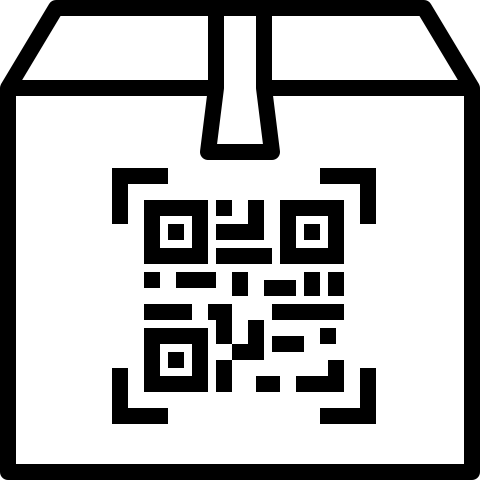
\includegraphics[width=4cm]{../assets/images/parcel.png}
		\end{column}
	\end{columns}
\end{frame}

%%%

\begin{frame}{Oracles on Bitcoin}
	\textbf{Example:} Alice and Bob want to bet on some event.\\
	\vspace{0.25cm}
	\uncover<2 ->{\textbf{Three possibilities:}}
	\begin{itemize}
		\vspace{0.1cm}
		\item<2->[1.] Both parties transfer their stake to the address of the oracle. The oracle then sends the prize to the winning party after the event has taken place.
		\begin{itemize}
			\item<2-> Problem: Control over funds lies solely with the oracle.
		\end{itemize}
		\vspace{0.2cm}
		\item<3->[2.] They create a 2-of-3 multisig transaction. Alice, Bob and the oracle each hold a key.
		\begin{itemize}
			\item<3-> Control distributed and Alice and Bob can overrule the oracle.
		\end{itemize}
		\vspace{0.2cm}
		\item<4->[3.] More than one oracle and use m-of-n multisig transaction. 
		\begin{itemize}
			\item<4-> Agents hold $\frac{m}{2}$ keys and m-1 oracles hold one key each.
			\item<4-> Any m-of-(2m-1) multisig implementation possible ($m$~has~to~be an even integer).
		\end{itemize}
	\end{itemize}
\end{frame}

%%%

\begin{frame}{Proof of Existence}
	\centering
	\begin{tikzpicture} 
		\uncover<+->{\node (img2) {
\includegraphics[width = 10cm, frame]{../assets/images/google1.PNG}};}
		\uncover<+->{\node (img3) at (img2) {
\includegraphics[width = 10cm, frame]{../assets/images/google2.PNG}};}
		\uncover<+->{\node (img4) at (img2) {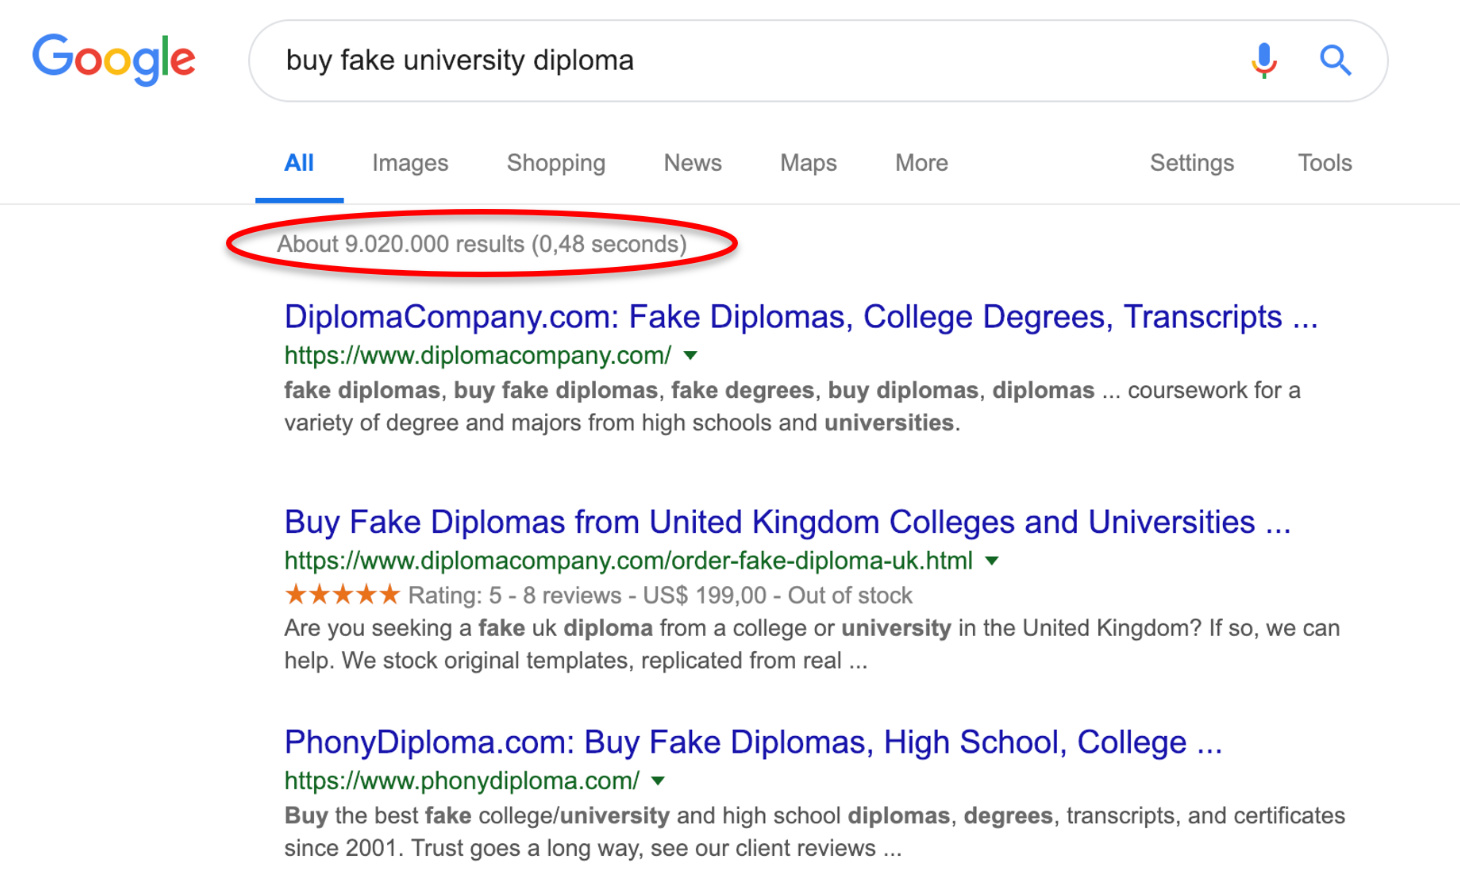
\includegraphics[width = 10cm, frame]{../assets/images/google3.PNG}};}
		\uncover<+->{\node (img5) at (img2) {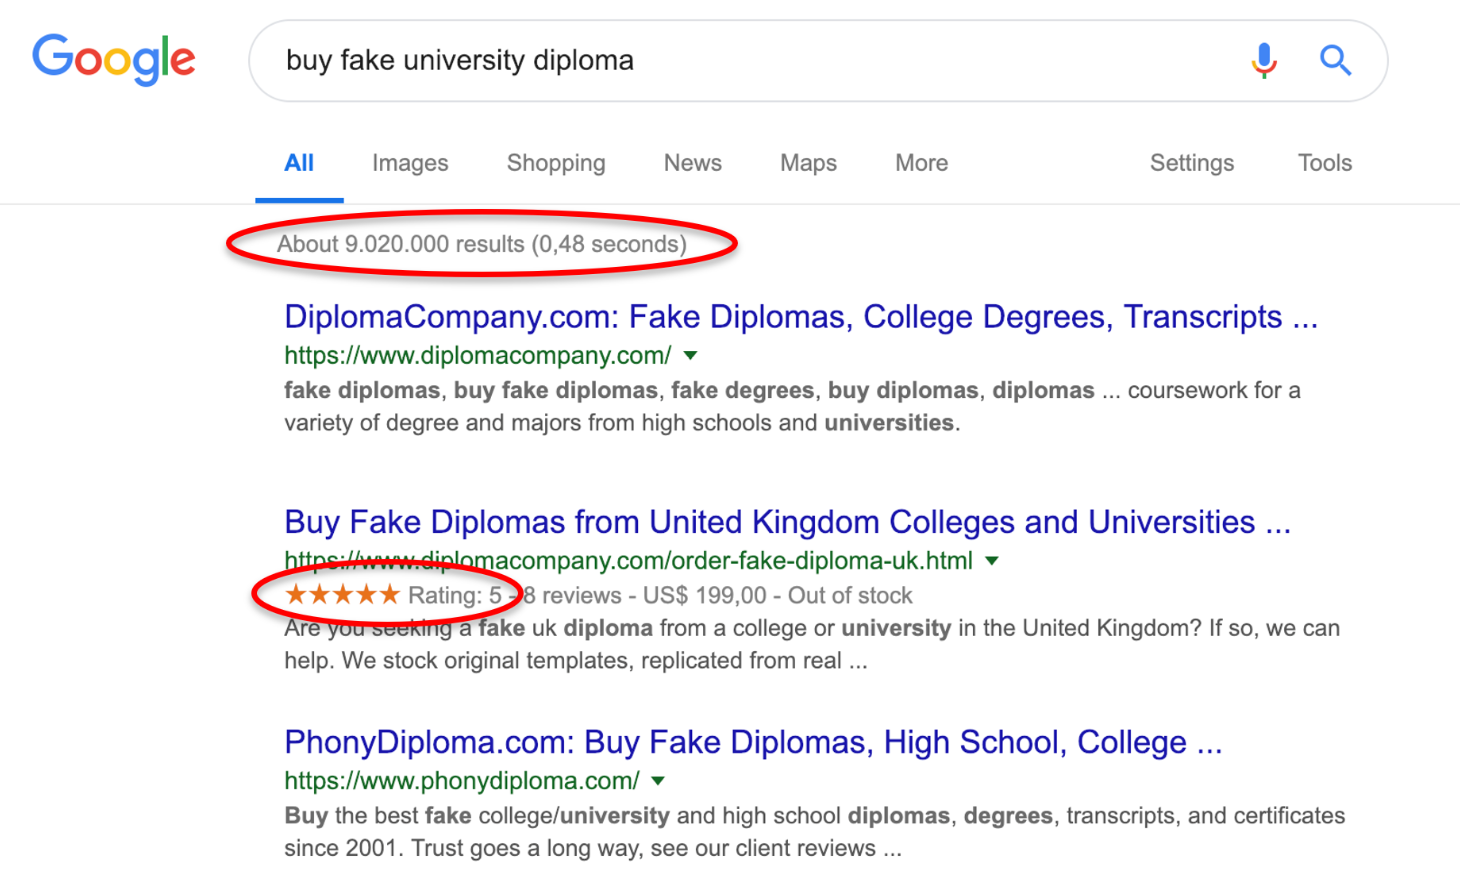
\includegraphics[width = 10cm, frame]{../assets/images/google4.PNG}};}
		\uncover<+->{\node (img7) at (img2) {
\includegraphics[width = 10cm, frame]{../assets/images/google6.PNG}};}
	\end{tikzpicture}
\end{frame}

%%%
\begin{frame}{Diplomas on the Blockchain}
	\begin{minipage}{\linewidth}
		\textbf{\large{Issuance:}}
			\begin{columns}
			\begin{column}{0.3\textwidth}
				\centering
				
\includegraphics[width=1.5cm]{../assets/images/diploma.png}\\
				University issues\\
				diploma
				\end{column}
			\begin{column}{0.05\textwidth}
				
\includegraphics[width=0.75cm]{../assets/images/big_arrow.png}
			\end{column}
			\begin{column}{0.3\textwidth}
				\centering
				
\includegraphics[width=1.5cm]{../assets/images/fingerprint.png}\\
				Computes hash value of diploma
			\end{column}
			\begin{column}{0.05\textwidth}
				
\includegraphics[width=0.75cm]{../assets/images/big_arrow.png}
			\end{column}
			\begin{column}{0.3\textwidth}
				\centering
				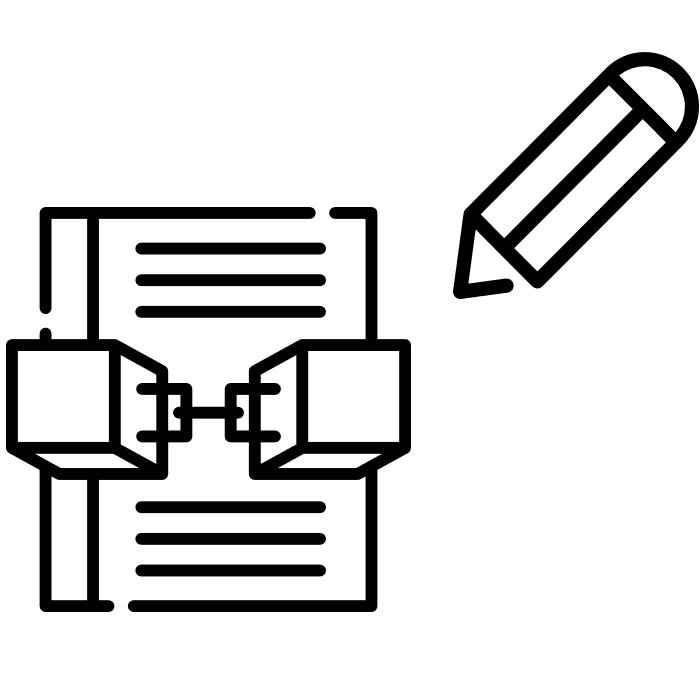
\includegraphics[width=1.5cm]{../assets/images/write_onchain.png}\\
				Saves hash value\\ on blockchain
			\end{column}
		\end{columns}
	\end{minipage}\vfill
	\vspace{0.5cm}
	\begin{minipage}{\linewidth}
	\textbf{\large{Verification:}}
	\begin{columns}
		\begin{column}{0.3\textwidth}
			\centering
			
\includegraphics[width=1.5cm]{../assets/images/receive_diploma.png}\\
			Potential employer receives diploma
		\end{column}
		\begin{column}{0.05\textwidth}
			
\includegraphics[width=0.75cm]{../assets/images/big_arrow.png}
		\end{column}
		\begin{column}{0.3\textwidth}
			\centering
			
\includegraphics[width=1.5cm]{../assets/images/fingerprint.png}\\
			Computes hash value of diploma
		\end{column}
		\begin{column}{0.05\textwidth}
			
\includegraphics[width=0.75cm]{../assets/images/big_arrow.png}
		\end{column}
		\begin{column}{0.3\textwidth}
			\centering
			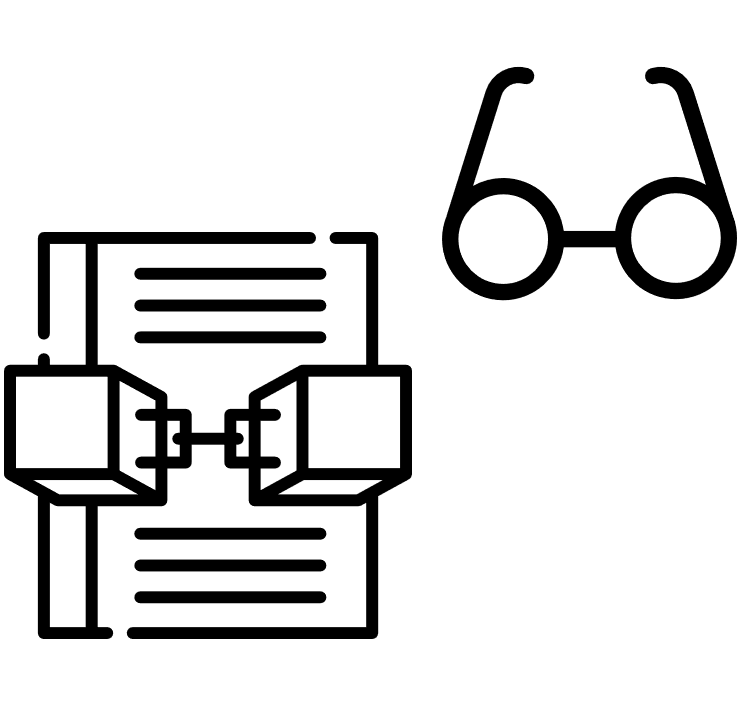
\includegraphics[width=1.5cm]{../assets/images/verify_onchain.png}\\
			Compares with on-chain hash value
		\end{column}
	\end{columns}
\end{minipage}
\end{frame}

%%%

\begin{frame}{Proof of Existence}
	\begin{columns}
		\begin{column}{0.4\textwidth}
			\begin{figure}
				\centering
				
\includegraphics[width=4cm, frame]{../assets/images/Diploma_unibas.PNG}
				\scriptsize{\href{https://cif.unibas.ch/en/events-projects/certificates/}{cif.unibas.ch/en/}}
			\end{figure}
		\end{column}
		\begin{column}{0.6\textwidth}
			\begin{itemize}
				\item<1 -> Certificate for Blockchain-related courses since 2018 
				\item<2 -> Roll-out for entire University of Basel coming soon
			\end{itemize}
		\end{column}
	\end{columns}
\end{frame}

%%%

\begin{frame}{Commit-Reveal}
	\begin{itemize}
		\item<1 -> Long known cryptographic primitive
		\item<2 -> First, commitment to a choice, without revealing it.
		\item<3 -> In second phase, choice is revealed.
		\item<4 -> Important: Commitment is secret and binding.\vspace{0.5cm}
		\item<5 -> Example:
		\begin{itemize}
			\item<5 -> Alice and Bob want to play rock-paper-scissors
			\item<6 -> Playing at the exact same time is difficult on blockchains
			\item<7 -> Solution: To commit to their choices, they hash them (salted) and save the hash value on-chain
			\item<8 -> Revealing their choices and the salts they can then determine the winner in a second step
		\end{itemize}
	\end{itemize}
\end{frame}

%%%

\begin{frame}[fragile]{Merkle Proofs}
	\begin{figure}
		\begin{minipage}[h]{0.55\linewidth}
			\centering
			
\includegraphics[width=4cm]{../assets/images/id.PNG}
		\end{minipage}%
		\hfill
		\begin{minipage}[h]{0.45\linewidth}
			\begin{itemize}
				\item<1 ->Alice has to proof a certain age
				\item<1 ->But Alice does not want to disclose other private information
			\end{itemize}
		\end{minipage}
	\end{figure}
	\vspace{-0.5cm}
	\begin{figure}
		\begin{minipage}[h]{0.55\linewidth}
			\hspace{-0.5cm}
			\begin{adjustbox}{width = 0.8\linewidth}
			\begin{lstlisting}[language=json,firstnumber=1]
				{
					"Name": "Alice",
					"SaltName": 103982023492,
					"DateOfBirth": "1/1/2000",
					"SaltDate": 787793837929,
					"PlaceOfBirth": "Basel",
					"SaltPlace": 989229104925
				}
			\end{lstlisting}
			\end{adjustbox}
			\centering
			\\[0.1cm] \scriptsize{Passport as a JSON object}
		\end{minipage}%
		\hfill
		\begin{minipage}[h]{0.45\linewidth}
			\begin{itemize}
				\item<2 ->Information is included in a merkle tree
				\item<2 ->Merkle root is saved on-chain by a trusted party (e.g. government)
			\end{itemize}
		\end{minipage}
	\end{figure}
\end{frame}

%%%

\begin{frame}{Merkle Proofs}
	\begin{figure}
		\centering
		\resizebox{9cm}{!}{%
		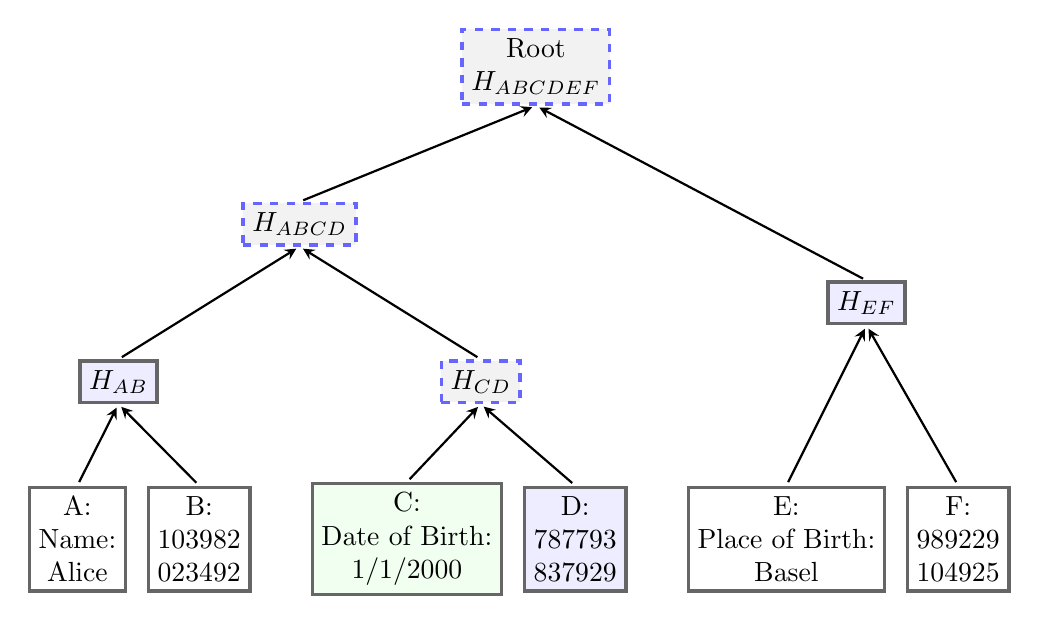
\begin{tikzpicture}[
			basicnode/.style={rectangle, draw=black!60, fill=white!5, very thick, minimum size=5mm},
			bluenode/.style={rectangle, draw=black!60, fill=blue!7, very thick, minimum size=5mm},
			greennode/.style={rectangle, draw=black!60, fill=green!6, very thick, minimum size=5mm},
			basicdotted/.style={rectangle, draw=blue!60, fill=black!5, very thick, dashed, minimum size=5mm},
			]
			%Nodes
			\node[bluenode, align=center] (startpoint) 	at (6,1) {D:\\ 787793\\837929};
			\node[basicnode, align=center] (PlaceOfBirth)	[right=0.75cm of startpoint] {E:\\ Place of Birth:\\ Basel};
			\node[basicnode, align=center] (F)	[right= 0.25cm of PlaceOfBirth] {F:\\ 989229\\ 104925};
			\node[greennode, align=center] (DateOfBirth)	[left= 0.25cm of startpoint] {C:\\ Date of Birth:\\ 1/1/2000};
			\node[basicnode, align=center] (B)	[left= 0.75cmof DateOfBirth] {B:\\ 103982\\ 023492};
			\node[basicnode, align=center] (Name)	[left= 0.25cm of B] {A:\\ Name:\\ Alice};
			
			\node[bluenode, align=center] (HAB) at (0.2,3) {$H_{AB}$};
			\node[basicdotted, align=center] (HCD) at (4.8,3) {$H_{CD}$};
			\node[bluenode, align=center] (HEF)	at (9.7,4) {$H_{EF}$};
			
			\node[basicdotted, align=center] (HABCD) at (2.5,5) {$H_{ABCD}$};
			\node[basicdotted, align=center] (HABCDEF)	at (5.5,7) {Root\\ $H_{ABCDEF}$};	
			
			%Lines
			\draw[-stealth,thick,shorten >=0.05cm,shorten <=0.05cm] (Name.north) -- (HAB.south);
			\draw[-stealth,thick, shorten >=0.05cm,shorten <=0.05cm] (B.north) -- (HAB.south);
			\draw[-stealth,thick, shorten >=0.05cm,shorten <=0.05cm] (DateOfBirth.north) -- (HCD.south);
			\draw[-stealth,thick, shorten >=0.05cm,shorten <=0.05cm] (startpoint.north) -- (HCD.south);
			\draw[-stealth,thick, shorten >=0.05cm,shorten <=0.05cm] (PlaceOfBirth.north) -- (HEF.south);
			\draw[-stealth,thick, shorten >=0.05cm,shorten <=0.05cm] (F.north) -- (HEF.south);
			
			\draw[-stealth,thick, shorten >=0.05cm,shorten <=0.05cm] (HAB.north) -- (HABCD.south);
			\draw[-stealth,thick, shorten >=0.05cm,shorten <=0.05cm] (HCD.north) -- (HABCD.south);
			\draw[-stealth,thick, shorten >=0.05cm,shorten <=0.05cm] (HABCD.north) -- (HABCDEF.south);
			\draw[-stealth,thick, shorten >=0.05cm,shorten <=0.05cm] (HEF.north) -- (HABCDEF.south);
		\end{tikzpicture}}
	\end{figure}
	\begin{itemize}
		\item<2 -> Alice provides C, D, $H_{AB}$ and $H_{EF}$
		\item<3 -> Authenticity can be verified with Merkle root ($H_{ABCDEF}$) 
	\end{itemize}
\end{frame}

%%%

\begin{frame}{Tokenization}
	\center
	\begin{block}{\textbf{Definition}}
		Non-native tokens are rivalrous digital units which entitle its current owner to (the delivery of) an asset or service.
	\end{block}
	\vspace{1cm}
	\uncover<2 ->{\begin{figure}
		\begin{minipage}[t]{0.45\linewidth}
			\center
			
\includegraphics[width=2cm]{../assets/images/house_1.png}
		\end{minipage}
		\hfill
		
\begin{tikzpicture}[remember picture, overlay]
			\node[above] at (-0.3, 1.6){\scriptsize{Counterparty Risk}};
			\fill[highlight] (-1.3, 0.6) -- (0, 0.6) -- (0, 0.1) -- (0.5, 0.85) -- (0, 1.6) -- (0, 1.2) -- (-1.3, 1.2) -- (-1.3, 0.6);
		\end{tikzpicture}
		\begin{minipage}[t]{0.45\linewidth}
			\center
			
\includegraphics[width=2.3cm]{../assets/images/token_house.png}
		\end{minipage}
	\end{figure}}
	\vspace{0.5cm}
	\begin{itemize}
		\item<3 ->Basically, every asset or promise can be tokenized
		\item<4 ->Differentiation between fungible and non-fungible tokens
	\end{itemize}
\end{frame}

%%%

\begin{frame}{Tokenization}
	\begin{columns}
		\begin{column}{0.6\textwidth}
			\textbf{Colored Coins}
			\begin{itemize}
				\item<2 -> External promise is attached to a Bitcoin UTXO
				\item<3 -> Additional output with meta data
				\item<4 -> Analogy: 
				\begin{itemize}
					\item<4 -> 5$\,$\$ bill
					\item<4 -> Promise is written on bill
					\item<4 -> Can freely circulate, including the promise
				\end{itemize}
			\end{itemize}
		\end{column}
		\begin{column}{0.4\textwidth}
			\vspace{-0.5cm}
			\begin{figure}
				\centering
				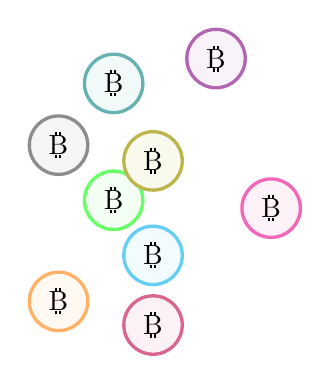
\begin{tikzpicture}[coloredCoin/.style={circle,  very thick, minimum size=5mm}]
					\node[coloredCoin, draw=green!60, fill=green!5] (green) at (1,1) {$\btc$};
					\node[coloredCoin, draw=magenta!60, fill=magenta!5] (magenta) at (3,0.9) {$\btc$};
					\node[coloredCoin, draw=teal!60, fill=teal!5] (teal) [above=0.7cm of green] {$\btc$};
					\node[coloredCoin, draw=darkgray!60, fill=darkgray!5] (darkgrey) at (0.3,1.7) {$\btc$};
					\node[coloredCoin, draw=orange!60, fill=orange!5] (orange) [below=1.2cm of darkgrey] {$\btc$};
					\node[coloredCoin, draw=olive!60, fill=olive!5] (olive) at (1.5,1.5) {$\btc$};
					\node[coloredCoin, draw=cyan!60, fill=cyan!5] (cyan) at (1.5,0.3) {$\btc$};
					\node[coloredCoin, draw=purple!60, fill=purple!5] [below=0.1cm of cyan] {$\btc$};
					\node[coloredCoin, draw=violet!60, fill=violet!5] at (2.3,2.8) {$\btc$};
				\end{tikzpicture}
			\end{figure}
		\end{column}
	\end{columns}
\end{frame}

%%%
\iffalse
\begin{frame}{Tokenization}
	\begin{columns}
		\begin{column}{0.65\textwidth}
			\textbf{Layer-based Tokens}
			\begin{itemize}
				\item<1 -> \texttt{OP\_RETURN} is used to save arbitrary data on-chain 
				\item<2 -> Transaction graph on a second layer is needed for interpretation
				\item<3 -> Analogy:
				\begin{itemize}
					\item<4 -> Transaction system based on newspapers
					\item<4 -> Promise (Token) is published in a encoded advertisement
					\item<4 -> External transaction graph interprets and registers transfer
				\end{itemize}
			\end{itemize}
		\end{column}
		\begin{column}{0.4\textwidth}
			\begin{figure}
				\centering
				
\includegraphics[width = 3.5cm]{../assets/images/newspaper.jpg}
			\end{figure}
		\end{column}
	\end{columns}
\end{frame}
\fi
%%%

\begin{frame}{Tokenization}	
	\begin{itemize}
		\item<1 ->\textbf{Colored Coins}
		\begin{itemize}
			\item<1 ->Use a fragment of a native Blockchain asset (UTXO) as a container
		\end{itemize}
		\vspace{1em}
		\item<2 ->\textbf{Layer-based Tokens}
		\begin{itemize}
			\item<2 -> Use metadata transactions (\texttt{OP\_RETURN}) and a separate transaction graph to create and track tokens
		\end{itemize}
		\vspace{1em}
		\item<3 ->\textbf{Smart Contract-based Token}
		\begin{itemize}
			\item<3 -> A dedicated smart contract creates and tracks states that represent token ownership. It maps tokens to current owner addresses.
		\end{itemize}
	\end{itemize}
\end{frame}

%%%

\begin{frame}{Smart Contracts}
	\begin{block}{\textbf{\textcolor{black}{Definition}}}
		"Smart contracts generally refer to small applications stored on a blockchain and executed in parallel by a large
		set of validators."\cite{schar2021defi}
		%ALTERNATIVE: A smart contract is a process which is secured by a distributed consensus protocol.
	\end{block}
	\begin{itemize}
		\item<2-> Definition not tied to a specific type of Blockchain
		\item<3-> Not smart, not a contract, not automated
	\end{itemize}
\end{frame}

%%%

\begin{frame}[fragile]{Smart Contracts}
	\begin{columns}
		\begin{column}{0.3\textwidth}
			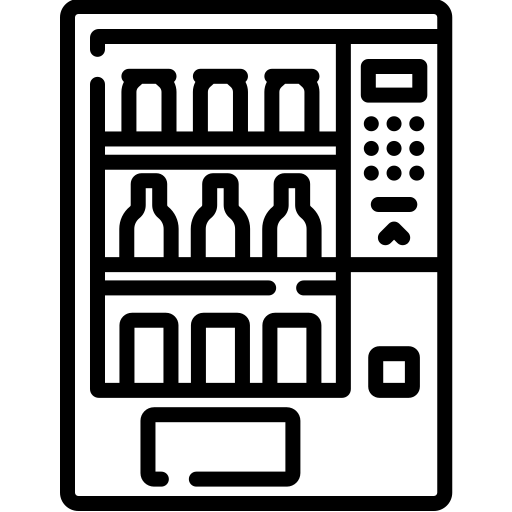
\includegraphics[width=1\textwidth]{../assets/images/vending-machine.png}
		\end{column}
		\begin{column}{0.5\textwidth}
			\begin{block}{\textcolor{black}{\textbf{Simple Vending Machine}}}
				\begin{lstlisting}[firstnumber=1,  xleftmargin=0pt, columns=fullflexible,language=Solidity] 
if(coin >= price){
	dispenseBeverage();
	returnChange(coin - price);
}else{
	print("insufficient funds");
}
				\end{lstlisting}
			\end{block}
		\end{column}
	\end{columns}
	\vspace{0.5cm}
	\uncover<2 ->{
		Vending Maschine:
		\begin{itemize}
			\item Plain code is not open source
			\item Execution environment is not visible
	\end{itemize}}
\end{frame}

%%%

\begin{frame}{Way too Short Intro to Ethereum}
	\begin{itemize}
		\item<1 ->Ethereum uses the account model instead of UTXO
		\begin{itemize}
			\item<1 ->One address per account
			\item<2 ->Nonce counts through numbers of transactions
		\end{itemize}
		\item<3 ->Externally Owned Accounts (EOA) controlled by private keys
		\item<4 ->Contract Accounts (CA) controlled by contract code
		\item<5 ->CAs are created by a transaction with 0 as recipient address. Transaction carries contract code.
		\item<6 ->More on smart contracts and Ethereum in next course at University of Basel (Autumn 2021)
	\end{itemize}
\end{frame}

%%%

\begin{frame}{Smart Contracts}
	\textbf{UTXOs as Smart Contracs:}
	\begin{itemize}
		\item<1-> By clever transaction design, one can create smart contracts on the Bitcoin Blockchain
		\item<2-> We already covered many building blocks e.g. MultiSig, SIGHASH types
		\item<3-> But, Bitcoin script is a limited scripting language (not Turing complete)
		\item<4-> The next lecture will give some examples for UTXO based smart contracts
	\end{itemize}
\end{frame}

%%%

\begin{frame}%[allowframebreaks]
	\frametitle{References}
	\bibliographystyle{amsplain}
	\bibliography{../assets/bib/refs}
\end{frame}

%%%
\end{document}